\documentclass[15pt,a5paper,reqno]{article}
\usepackage{hyperref}
\usepackage[warn]{mathtext}
\usepackage[utf8x]{inputenc}
\usepackage{amssymb, amsmath, multicol}
\usepackage[russian]{babel}
\usepackage{graphicx}
\usepackage[shortcuts,cyremdash]{extdash}
\usepackage{wrapfig}
\usepackage{floatflt}
\usepackage{lipsum}
\usepackage{verbatim}
\usepackage{concmath}
\usepackage{euler}
\usepackage{xcolor}
\usepackage{etoolbox}
\usepackage{fancyhdr}
\usepackage{subfiles}
\usepackage{enumitem}
\usepackage{amsthm}
\usepackage{indentfirst}
\usepackage{import}

\DeclareMathOperator{\sign}{sign}

\RequirePackage[ left     = 1.5cm,
  right    = 1.5cm,
  top      = 2.0cm,
  bottom   = 1.25cm,
  includefoot,
  footskip = 1.25cm ]{geometry}
\setlength    {\parskip}        { .5em plus .15em minus .08em }
%\setlength    {\parindent}      { .0em }
\renewcommand {\baselinestretch}{ 1.07 }

\fancyhf{}

\renewcommand{\footrulewidth}{ .0em }
\fancyfoot[C]{\texttt{\textemdash~\thepage~\textemdash}}
\fancyhead[R]{\hfilШурыгин, Тяжкороб, Широкова}

\makeatletter
\patchcmd\l@section{%
  \nobreak\hfil\nobreak
}{%
  \nobreak
  \leaders\hbox{%
    $\m@th \mkern \@dotsep mu\hbox{.}\mkern \@dotsep mu$%
  }%
  \hfill
  \nobreak
}{}{\errmessage{\noexpand\l@section could not be patched}}
\makeatother
\parindent = 1cm % отступ при красной строке⏎
\pagestyle{fancy}    
\renewcommand\qedsymbol{$\blacksquare$}

\newcommand{\when}[2]{
  \left. #1 \right|_{#2} \hspace
}
\renewcommand{\kappa}{\varkappa}
\RequirePackage{caption2}
\renewcommand\captionlabeldelim{}
\newcommand*{\hm}[1]{#1\nobreak\discretionary{}

\DeclareSymbolFont{T2Aletters}{T2A}{cmr}{m}{it}
{\hbox{$\mathsurround=0pt #1$}}{}}
% Цвета для гиперссылок
\definecolor{linkcolor}{HTML}{000000} % цвет ссылок
\definecolor{urlcolor}{HTML}{799B03} % цвет гиперссылок
 
\hypersetup{pdfstartview=FitH,  linkcolor=linkcolor,urlcolor=urlcolor, colorlinks=true}


%\setcounter{secnum[utf8x]depth}{0}

\begin{document}

% НАЧАЛО ТИТУЛЬНОГО ЛИСТА
\begin{center}
  {\small ФЕДЕРАЛЬНОЕ ГОСУДАРСТВЕННОЕ АВТОНОМНОЕ ОБРАЗОВАТЕЛЬНОЕ\\ УЧРЕЖДЕНИЕ ВЫСШЕГО ОБРАЗОВАНИЯ\\ МОСКОВСКИЙ ФИЗИКО-ТЕХНИЧЕСКИЙ ИНСТИТУТ\\ (НАЦИОНАЛЬНЫЙ ИССЛЕДОВАТЕЛЬСКИЙ УНИВЕРСИТЕТ)\\ ФИЗТЕХ-ШКОЛА РАДИОТЕХНИКИ И КИБЕРНЕТИКИ}\\
  \hfill \break
  \hfill \break
  \hfill \break
  \Huge{Активные фильтры}\\
\end{center}

\hfill \break
\hfill \break
\hfill \break
\hfill \break
\hfill \break
\hfill \break

\begin{flushright}
  \normalsize{Работу выполнили:}\\
  \normalsize{\textbf{Шурыгин Антон Алексеевич, группа Б01-909 \\
                      Тяжкороб Ульяна Владимировна, группа Б01-909   \\   
                      Широкова Ксения Михайловна, группа Б01-909}}\\
\end{flushright}

\begin{center}
  \normalsize{\textbf{Долгопрудный, 2021}}
\end{center}


\thispagestyle{empty} % выключаем отображение номера для этой страницы

% КОНЕЦ ТИТУЛЬНОГО ЛИСТА

\newpage
\thispagestyle{plain}
\tableofcontents
\thispagestyle{plain}
\newpage



\section{Звенья первого порядка.}

\subsection{}

\begin{figure}[h!]
  \centering
  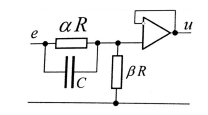
\includegraphics[width=0.4\linewidth]{pics/pic1.png}
  \caption{Пропорционально дифференцирующее звено.}
  \label{}
\end{figure}

\begin{figure}[h!]
  \centering
  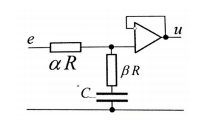
\includegraphics[width=0.4\linewidth]{pics/pic2.png}
  \caption{ Пропорционально интегрирующее звено.}
  \label{}
\end{figure}


Измерим уровни подавления на частоте $f_0$ и в полосах задержания для пропорционально интегрирующей и дифференцирующей цепей с полюсом в точке s = $\frac{p}{\omega_0} = -1$,
$f_0 = \frac{\omega_0}{2\pi} = 10k$ и нулями в точках $s = -2, s = -\frac{1}{2}$. Измерим уровни подавления на частоте $f_0$ и
в полосах задержания.
\begin{equation*}
    \delta = \frac{\beta}{\beta + \alpha} = \frac{1}{2}  \text{-− уровень подавления в полосе задержания} 
\end{equation*}
Подавление на частоте $f_0$ = 10k:

\begin{equation*}
    \frac{4}{5} \text{-интегрирующее звено,} \\
    \\
    \frac{1}{5} \text{-дифференцирующее звено.}
\end{equation*}

\subsection{}

Изменим номиналы резисторов в схемах так, чтобы сохранив положения полюсов,
переместить нули в точки $s = -4$, $s = -\frac{1}{4}$.
\par
$\delta = \frac{1}{4}$ - уровень подавления в полосе задержания. Уровень подавления на частоте $f_0$: $\frac{1}{2}$ - интегрирующая, $\frac{3}{20}$ - дифференцирующая.


\subsection{}
Откроем модель реального интегратора с частотой единичного усиления $f_0 = \frac{1}{2\pi RC} = 10k $ и усилением $K = \frac{R_k}{R}$, $R_k = [20k, 640k | \log{2}]$.

\begin{figure}[h!]
  \centering
  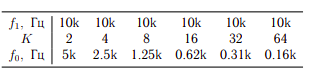
\includegraphics[width=0.8\linewidth]{pics/pic3.png}
  \caption{}
  \label{}
\end{figure}

\begin{figure}[h!]
  \centering
  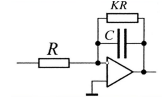
\includegraphics[width=0.4\linewidth]{pics/pic4.png}
  \caption{Реальный интегратор.}
  \label{}
\end{figure}


\begin{equation*}
    f_1 = f_0K \text { - соотношение выполняется}
\end{equation*}

\subsection{}

Подключим источник $step$ единичного перепада. Изучим переходные характеристики интегратора $ h \frac{\tau}{\tau_1})$, $\tau_1$ = $RC$ = 15.92$\mu$.

Варьируем $R_k = [20k, 640k| log 2]$ и оцениваем значения ошибок интегрирования в точках $\frac{\tau}{\tau_1} = \frac{K}{2}$

Подключим источник pulse. Изучим переходные характеристики интегратора $ h (\frac{t}{\tau_1})$, $\tau_1 = RC = 15.92µ$. 

Варьируем $R_k = [20k, 640k| log 2]$ и оцениваем значения ошибок интегрирования в точках  $\frac{\tau}{tau_1} = \frac{K}{2}$. 

Результат занесен в таблицу.

\begin{table}[h!]
	\centering
	\begin{tabular}{| c | c | c |}
\hline

$\frac{\tau}{\tau_1}$ & $R_k, k$ & $error$ \\
\hline
$1$ & $20$ & $0.185$\\
\hline
$2$ & $40$ & $0.384$\\
\hline
$4$ & $80$ & $0.781$\\
\hline
$8$ & $160$ & $1.578$\\
\hline
$16$ & $320$ & $3.177$\\
\hline
$32$ & $640$ & $6.4$\\
\hline
\end{tabular}

	\caption{Ошибка интегрирования при варьировании $R_k$ (step)}
	\label{nu1}
\end{table}

\begin{table}[h!]
	\centering
	\begin{tabular}{| c | c | c |}
\hline

$\frac{\tau}{\tau_1}$ & $R_k, k$ & $error$ \\
\hline
$1$ & $20$ & $0.582$\\
\hline
$2$ & $40$ & $1.178$\\
\hline
$4$ & $80$ & $2.356$\\
\hline
$8$ & $160$ & $4.722$\\
\hline
$16$ & $320$ & $9.456$\\
\hline
$32$ & $640$ & $18.927$\\
\hline
\end{tabular}

	\caption{Ошибка интегрирования при варьировании $R_k$ (pulse)}
	\label{nu1}
\end{table}

\newpage
%------------------------------------------------

\section{Активные звенья с двойным Т-мостом}


\begin{figure}[h!]
    \centering
    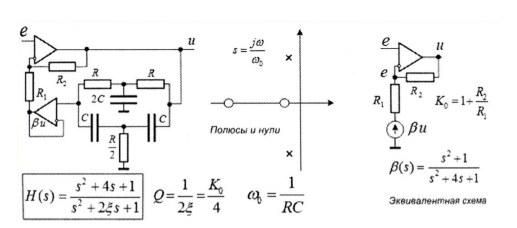
\includegraphics[width=1\linewidth]{pics/pic5.png} 
    \caption{Полосовой фильтр с двойным Т - мостом.}
\end{figure}

\subsection{}

 Откроем модель полосового фильтра c $f_0 = 10k$, $K_0 = 20$. Измерим
усиление на частоте $f_0$ и полосу $\Delta f$ по уровню -3dB. Получаем $K_0 = 20.92$,
$\Delta f = 1.93$ ($R_2 = 20k$).

\begin{figure}[h!]
    \centering
    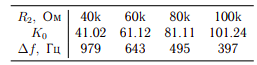
\includegraphics[width=0.4\linewidth]{pics/pic6.png}
    \caption{Зависимость пикового усиления и ширины полосы от $R_2$.}
\end{figure}

\subsection{}

Изучим поведение фильтра при разбалансировании моста варьированием $R_5$. Снимем зависимость от $R_5$ пикового усиления.
\begin{figure}[h!]
    \centering
    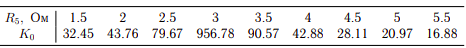
\includegraphics[width=0.8\linewidth]{pics/pic7.png}
    \caption*{Зависимость пикового усиления от $R_5$.}
\end{figure}
\subsection{}
Измерим уровни скачка в нуле и первого выброса: уровень скачка - 1В при $R_5$ =
5k Ом.
Оценим значение $R_5$, при котором фильтр теряет устойчивость.

\begin{figure}[h!]
    \centering
    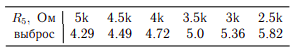
\includegraphics[width=0.5\linewidth]{pics/pic8.png}
\end{figure}


\subsection{}

Откроем модель режекторного фильтра c $f_0 = 10k$, $\gamma = 0.1$.

\begin{figure}[h!]
    \centering
    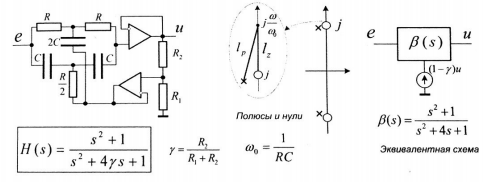
\includegraphics[width=1\linewidth]{pics/pic9.png}
    \caption{Режекторный фильтр с двойным Т - мостом.}
\end{figure}

Измерим ширину полосы режекции $\Delta f$ по уровню 0.7 = −3dB. Получим: $\Delta f$ = 4.07 кГц.

\subsection{}


Измерим уровни скачка в нуле и первого выброса. Получим: уровень скачка - 1В, первый выброс - 697.5 мВ.

\newpage

\section{Звенья Саллена-Ки.}

\begin{figure}[h!]
    \centering
    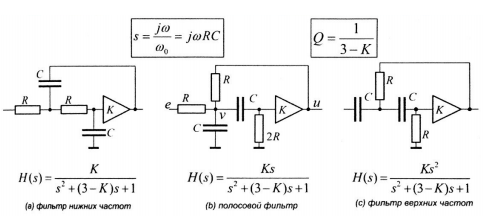
\includegraphics[width=1\linewidth]{pics/pic10.png}
    \caption*{Звенья Саллена-Ки.}
\end{figure}

\subsection{}
Откроем модель звеньев Саллена-Ки с частотой $f_0 = 10k$ и добротностью $Q = 1$.
Измерим значения коэффициентов передачи при $f = f_0$. Получим:

\begin{equation*}
    K_0 = 2, \space k_{lp} = 29.44, \space K_{hp} = 28.485, \space K_{bp} = 28.898
\end{equation*}

\subsection{}

Откроем модель с фильтрами Баттерворта верхних и нижних частот
порядка $n = 3$ на частоту среза $f_0 = 10k$. Измерим скорости спада в dB на октаву и
затухания на частотах $f_0/2$, $2f_0$:
\par
ВЧ: затухание на $f_0/2$ : −18 dB, скорость спада −15 $\frac{dB}{\text{дек}}$
дек
\par
НЧ: затухание на $2f_0$ : −18 dB, скорость спада 15 $\frac{dB}{\text{дек}}$
дек
.
\medskip
\par
Измерим уровни затухания фильтров Чебышева на частотах $f_0/2$, $2f_0$:
\par
ВЧ: затухание на $f_0/2$ : −30 dB, скорость спада −18 $\frac{db}{\text{деб}}$
дек
\par
НЧ: затухание на $2f_0$ : −30 dB, скорость спада 18 $\frac{db}{\text{деб}}$
дек
.

\subsection{}
Откроем прототип , реализуем 4-полюсной полосовой фильтр Чебышева
с  $f_0 = 10k$, $\epsilon = 1$, $Q = \frac{f_0}{\Delta f} = 6$. Измерим затухания на частотах $f_0/2$, $2f_0$, $f_0/10$, $10f_0$.
%------------------------------------------------

\begin{figure}[h!]
    \centering
    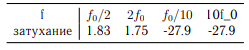
\includegraphics[width=0.4\linewidth]{pics/pic11.png}
\end{figure}

\section{ Звенья с двойной обратной связью.}
\subsection{}

Полосовое звено с $f_0 = 5k$, $K_0 = 5$, $Q = 15$

\begin{figure}[h!]
    \centering
    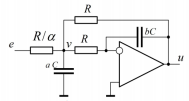
\includegraphics[width=0.3\linewidth]{pic12.png}
\end{figure}

$f_{max} = 4.980k$, $\Delta f = 338$ - ширина полосы по уровню 0.7.
$Q=\frac{f_{max}}{\Delta f} = 14.7$, $QK_0 = 73.5$ - пиковое усиление.

Построим график зависимости частоты пика от $R_2$


\begin{figure}[h!]
    \centering
    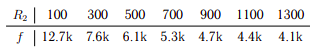
\includegraphics[width=0.5\linewidth]{pic13.png}
\end{figure}


\begin{figure}[h!]
    \centering
    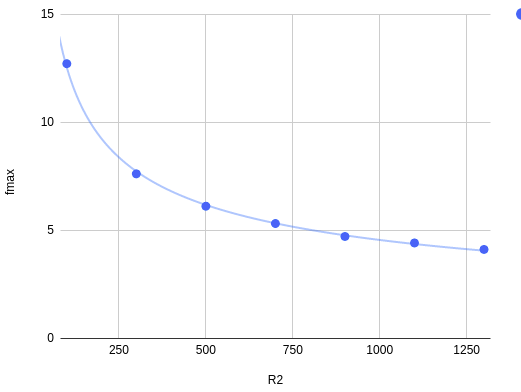
\includegraphics[width=0.6\linewidth]{pic14.png}
\end{figure}


На практике:


\begin{equation*}
	f_{max} = 5.05k, \hfill K_0 = 5.77
\end{equation*}


\section{Полосовое звено на сдвоенном усилителе.}

\subsection{}
\begin{figure}[h!]
    \centering
    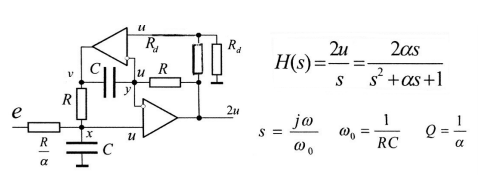
\includegraphics[width=0.8\linewidth]{pic15.png}
    \caption*{Полосовой фильтр на сдвоенном операционном усилителе.}
\end{figure}


По частотной характеристике звена оценим его параметры:$f_0 =
10k$, $Q = 9.7$. Измерим значение добротности при $R_2 = 6400k$.

\subsection{}

Измерим частоту и уровень пика при $R_5 = 1.11k$ ($\gamma = \frac{R_5}{R_4 + R_5} = 0.1$): $f = 31.415k$, уровень пика - 24.079


\begin{figure}[h!]
    \centering
    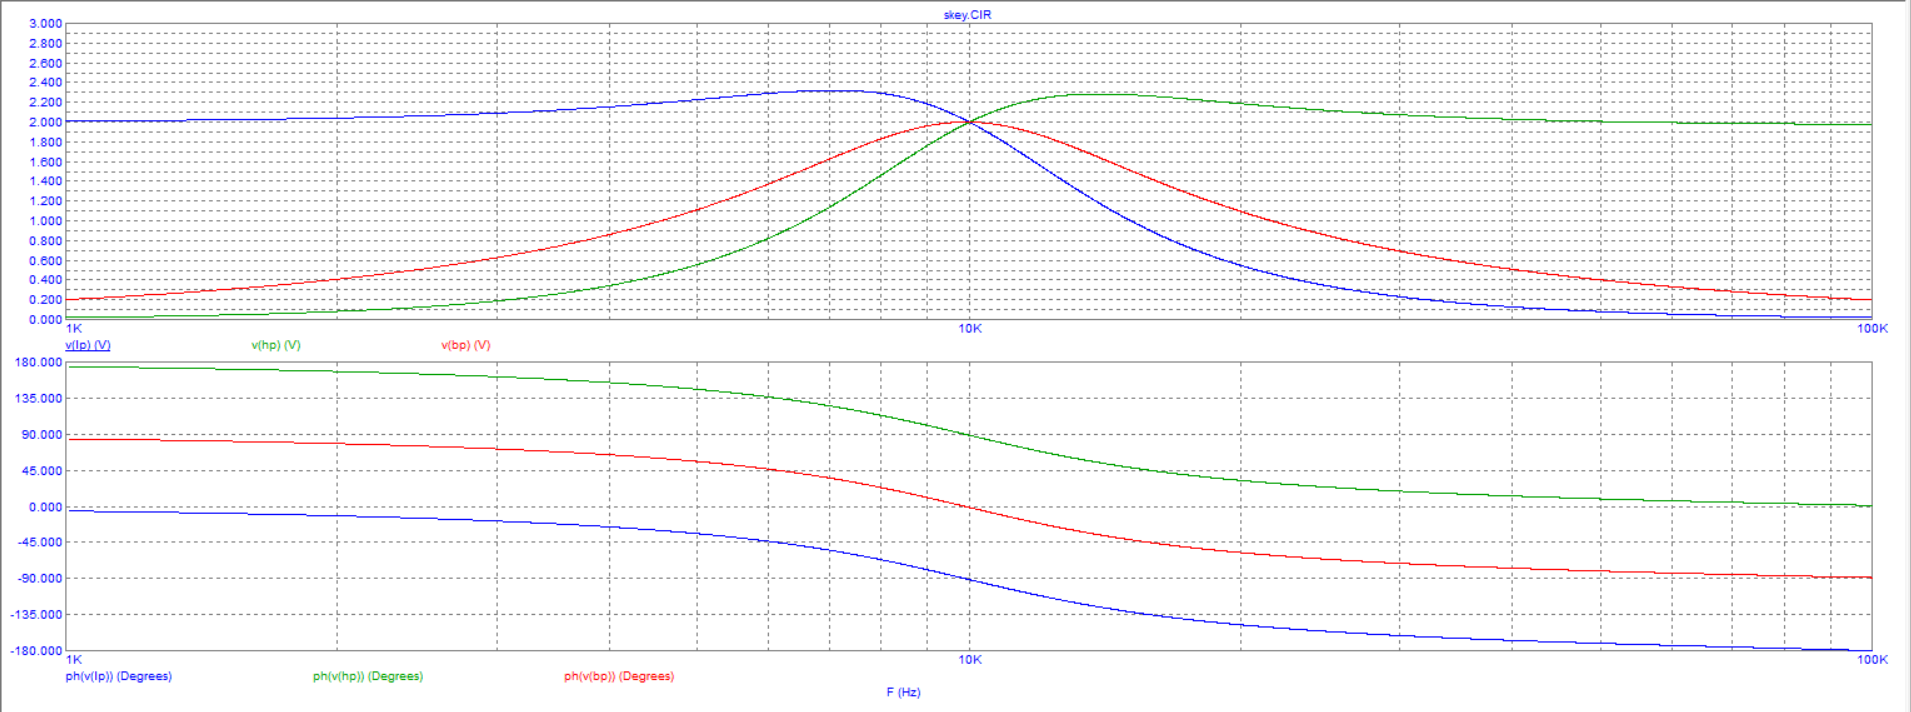
\includegraphics[width=12cm]{pics/point4.png}
    \caption{}
    \label{Задание 4 пункт 1. частотные характеристики фнч фвч и пф}
\end{figure}



\begin{figure}[h!]
    \centering
    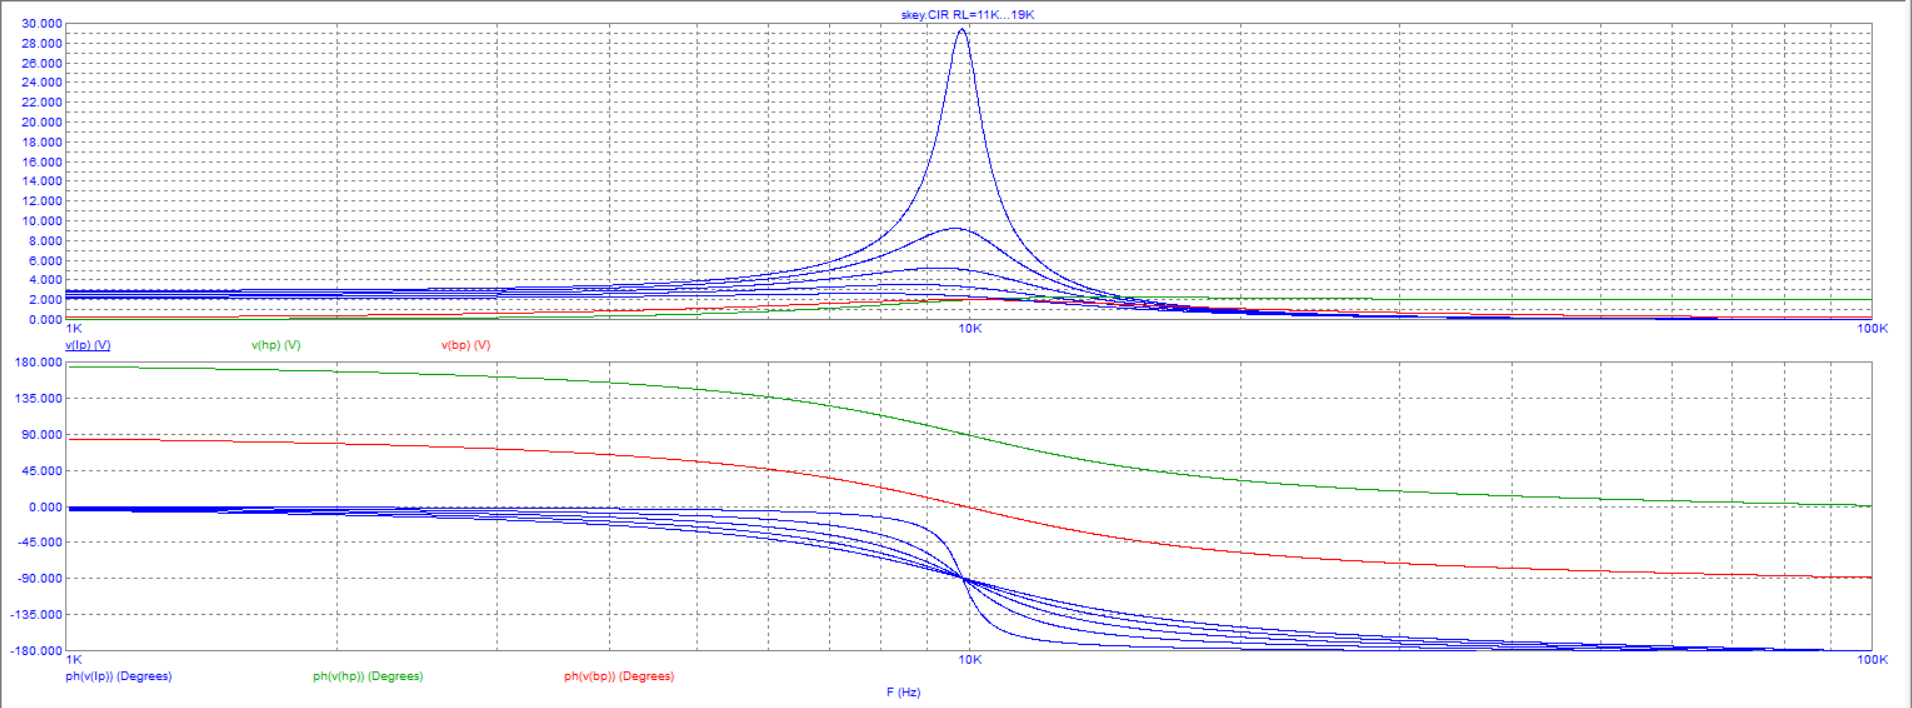
\includegraphics[width=12cm]{pics/point4_1_var1.png}
    \caption{Варьирование $R_l = [11K, 19K | 2K]$}
    \label{}
\end{figure}



\begin{figure}[h!]
    \centering
    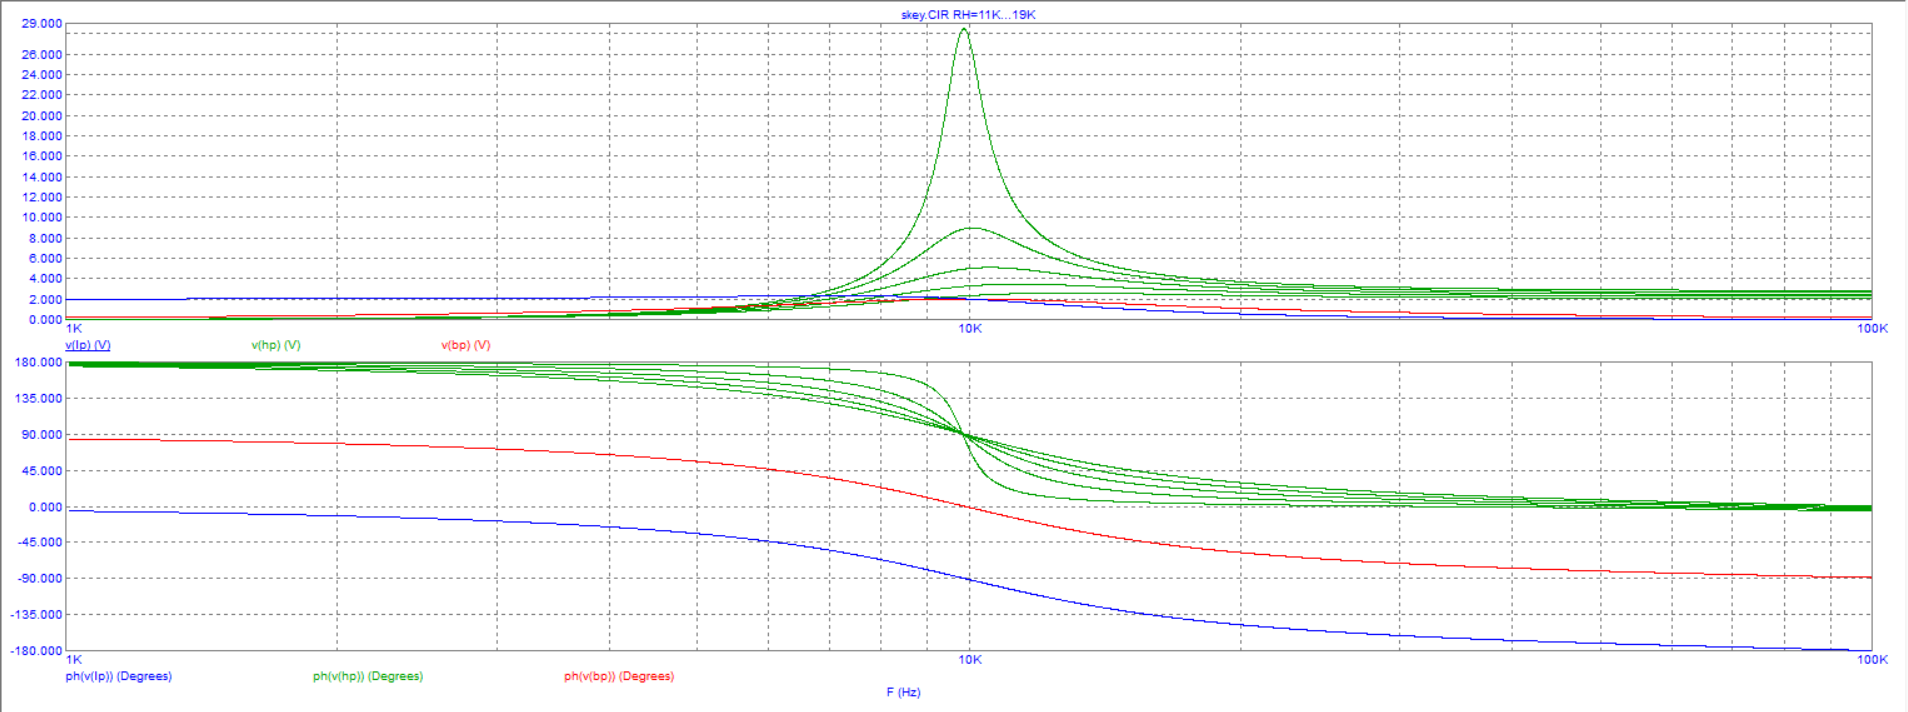
\includegraphics[width=12cm]{pics/point4_1_var2.png}
    \caption{Варьирование $R_H = [11K, 19K | 2K]$}
    \label{}
\end{figure}




\begin{figure}[h!]
    \centering
    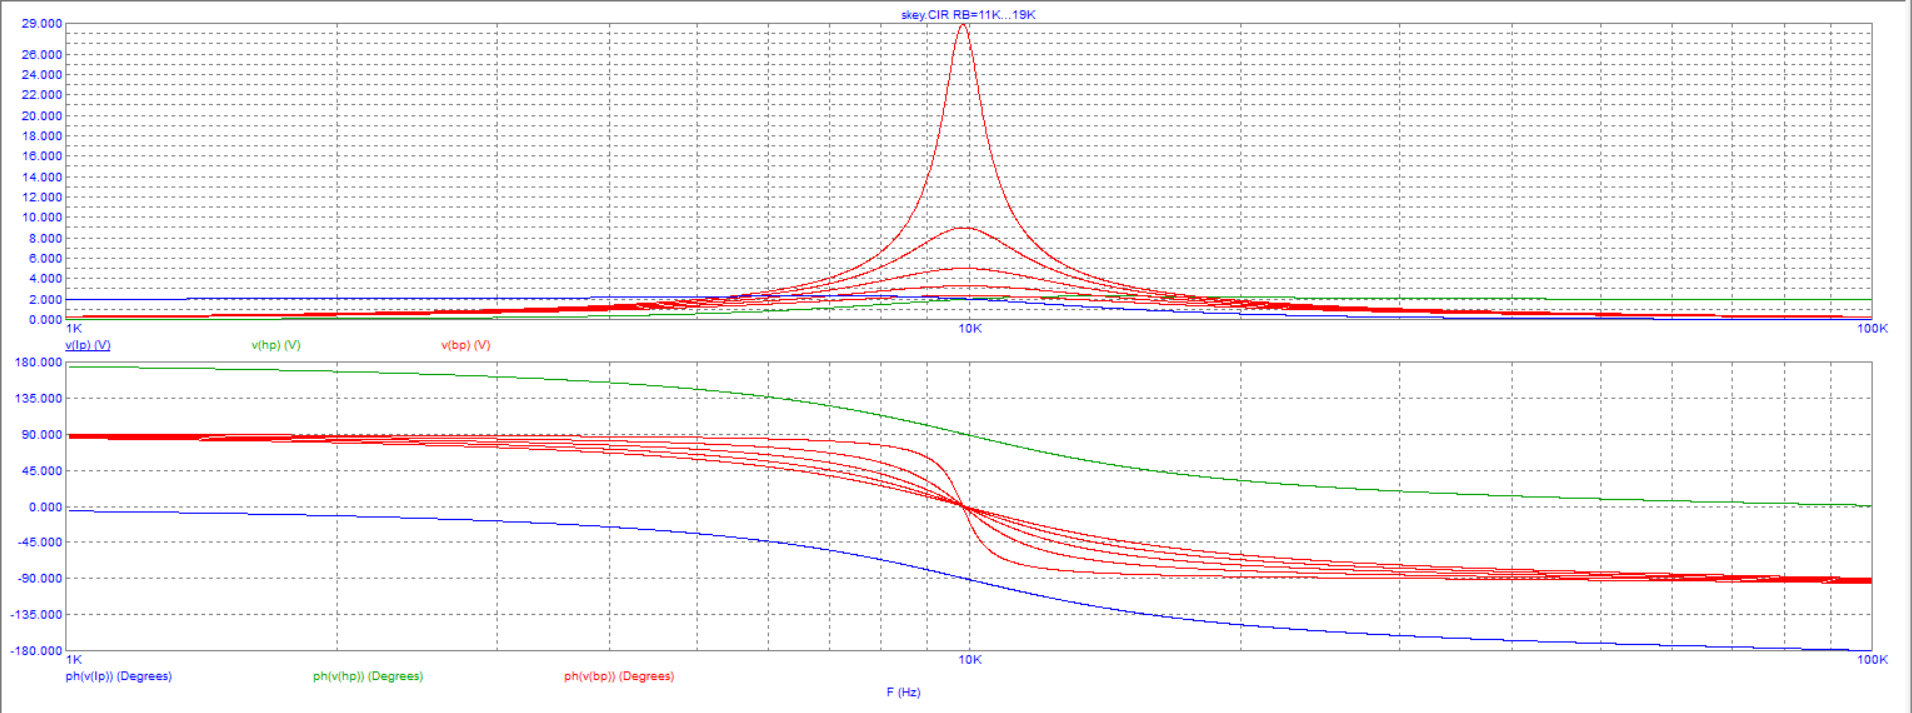
\includegraphics[width=12cm]{pics/point4_1_var3.png}
    \caption{Варьирование $R_B  = 11K, 19K | 2K]$}
    \label{}
\end{figure}




\begin{figure}[h!]
    \centering
    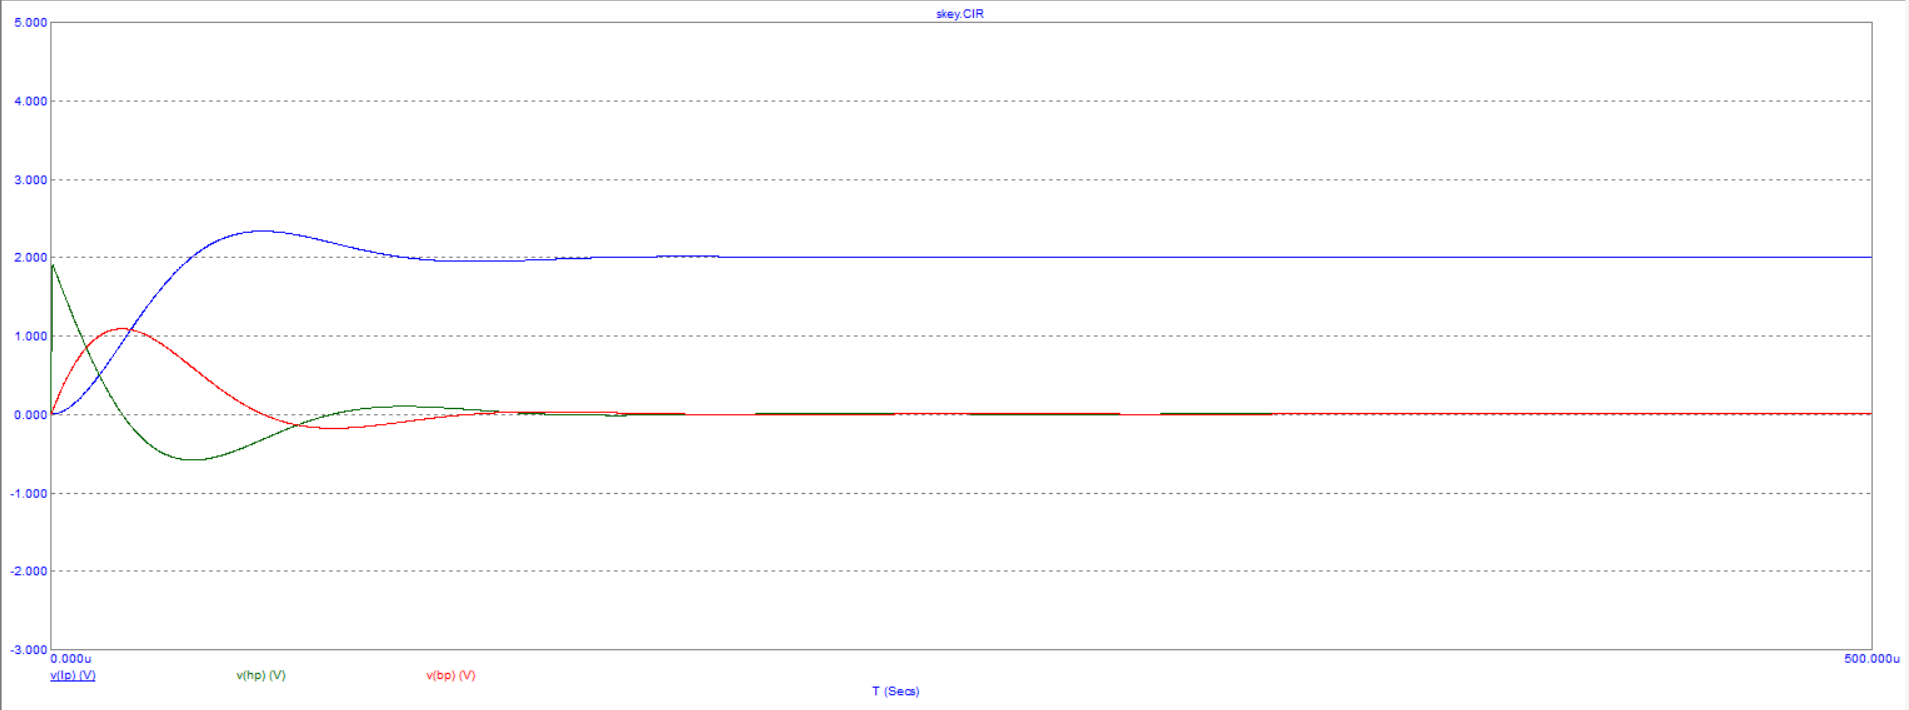
\includegraphics[width=12cm]{pics/point4_2.png}
    \caption{Варьирование $R_B  = 11K, 19K | 2K]$}
    \label{}
\end{figure}


\begin{figure}[h!]
    \centering
    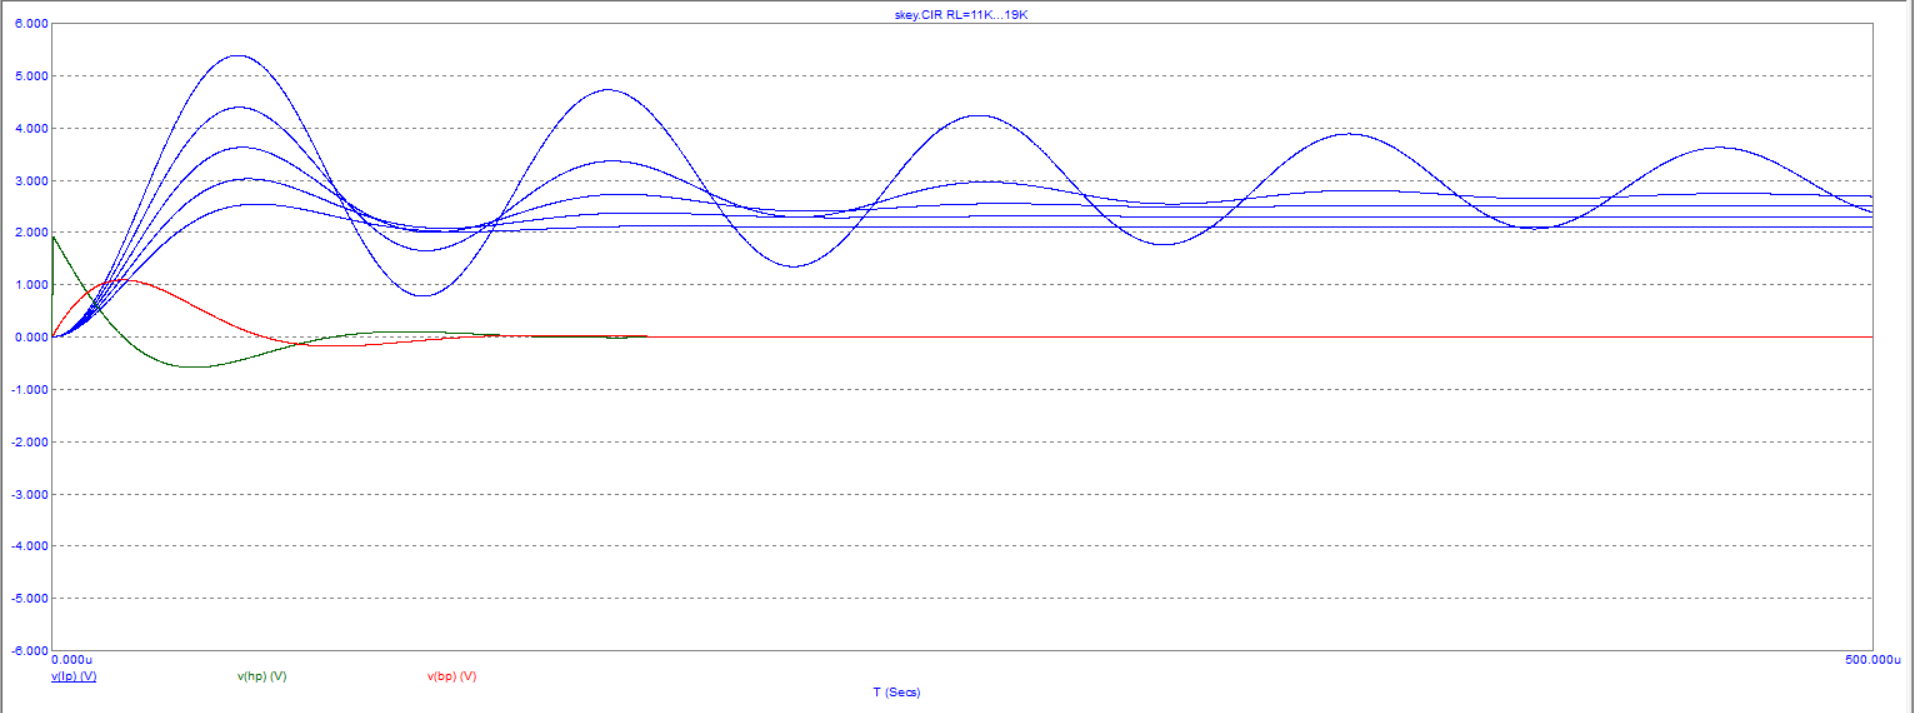
\includegraphics[width=12cm]{pics/point4_2_var1.png}
    \caption{Варьирование $R_B  = 11K, 19K | 2K]$}
    \label{}
\end{figure}



\begin{figure}[h!]
    \centering
    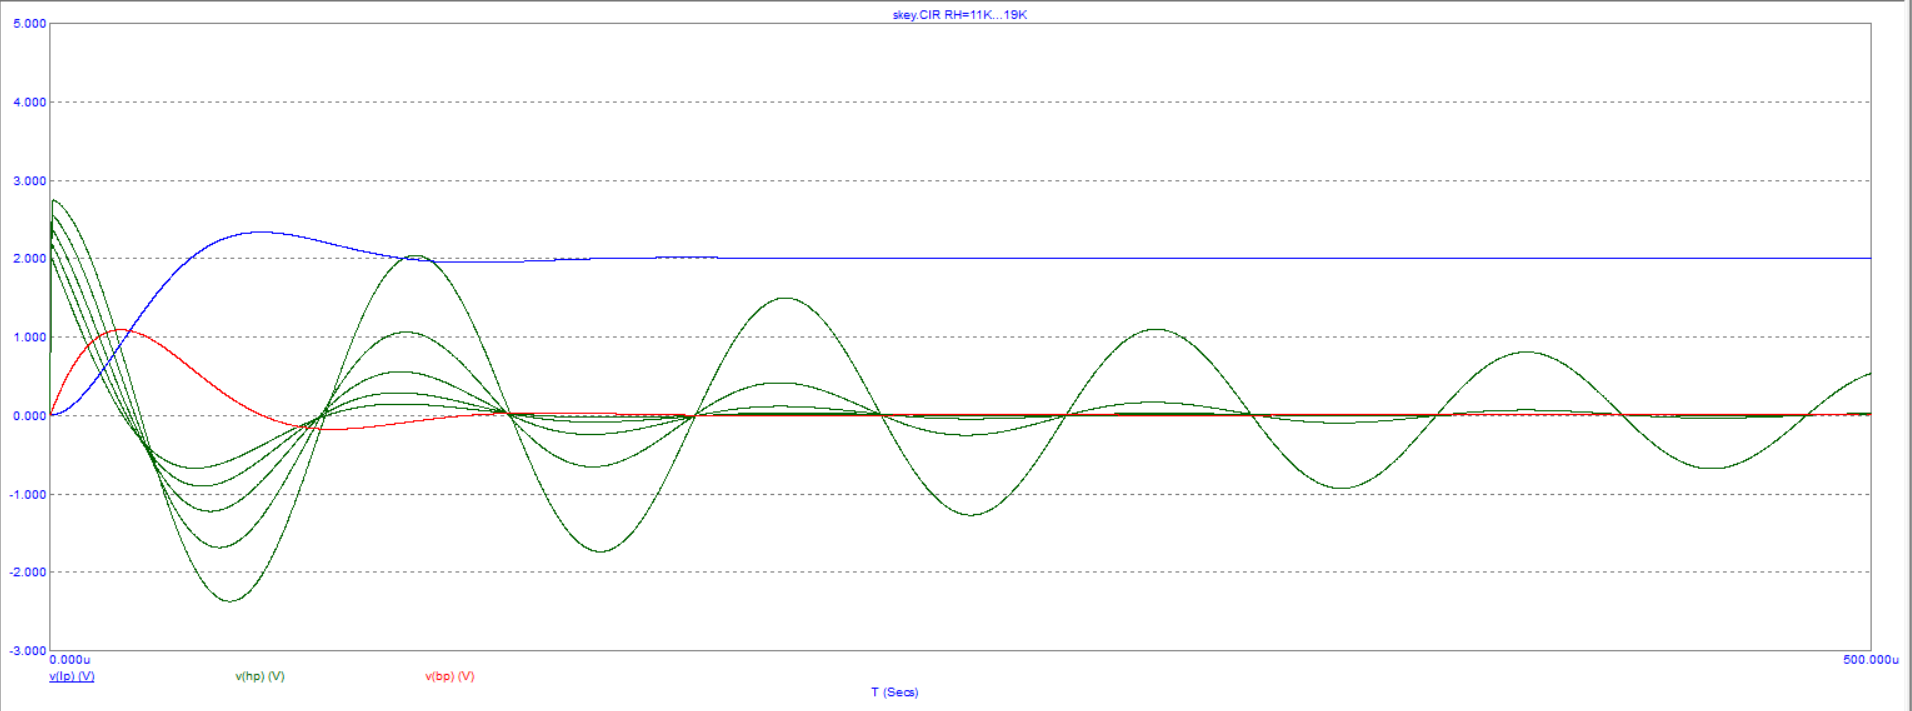
\includegraphics[width=12cm]{pics/point4_2_var2.png}
    \caption{Варьирование $R_B  = 11K, 19K | 2K]$}
    \label{}
\end{figure}


\begin{figure}[h!]
    \centering
    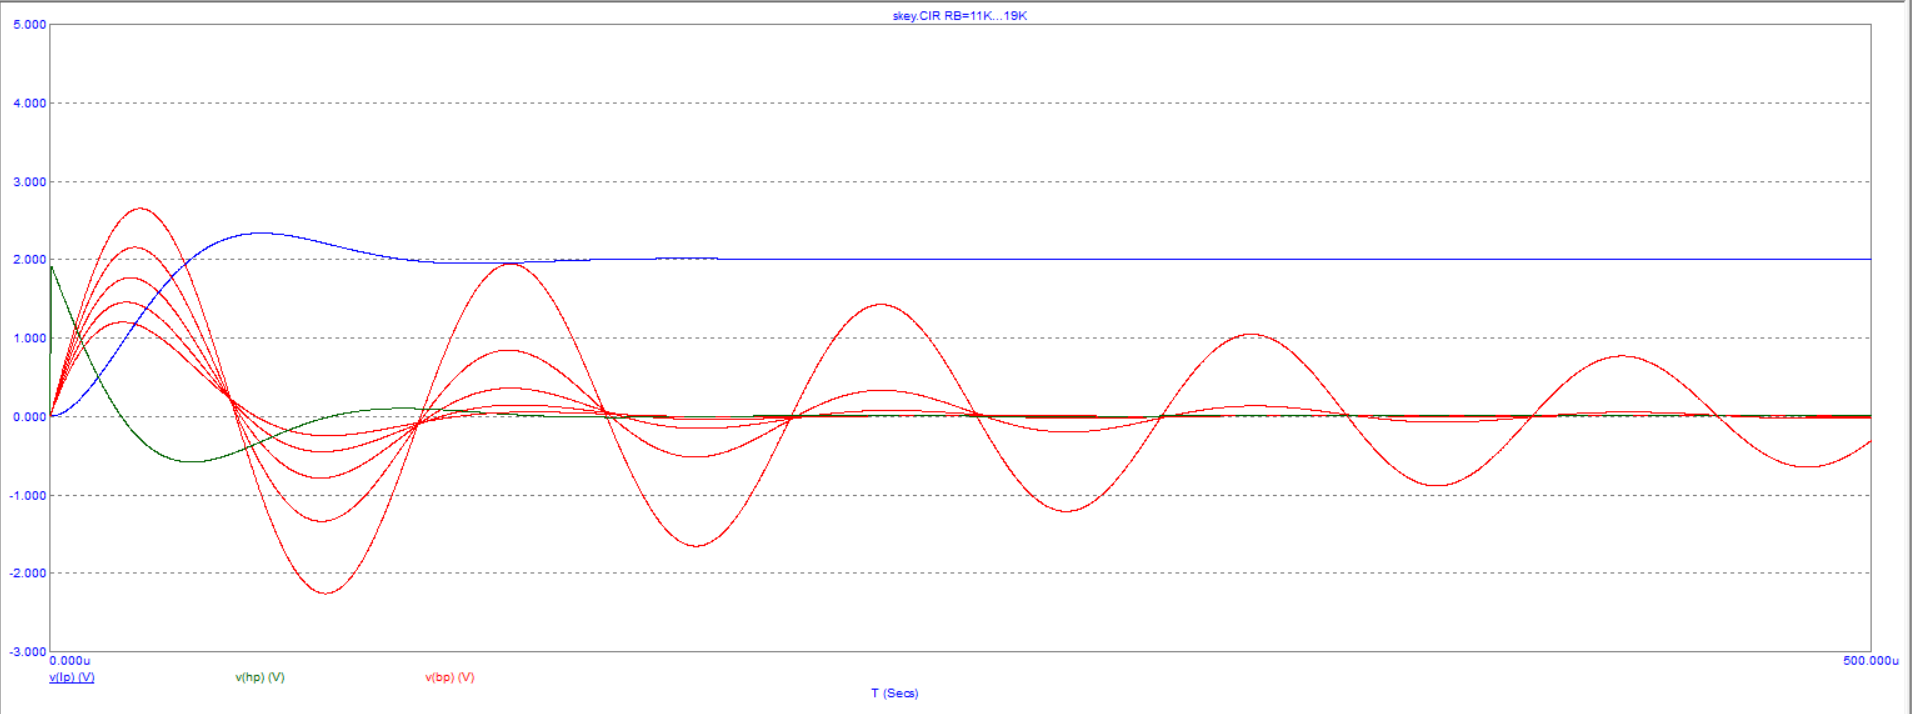
\includegraphics[width=12cm]{pics/point4_2_var3.png}
    \caption{Варьирование $R_B  = 11K, 19K | 2K]$}
    \label{}
\end{figure}


\begin{figure}[h!]
    \centering
    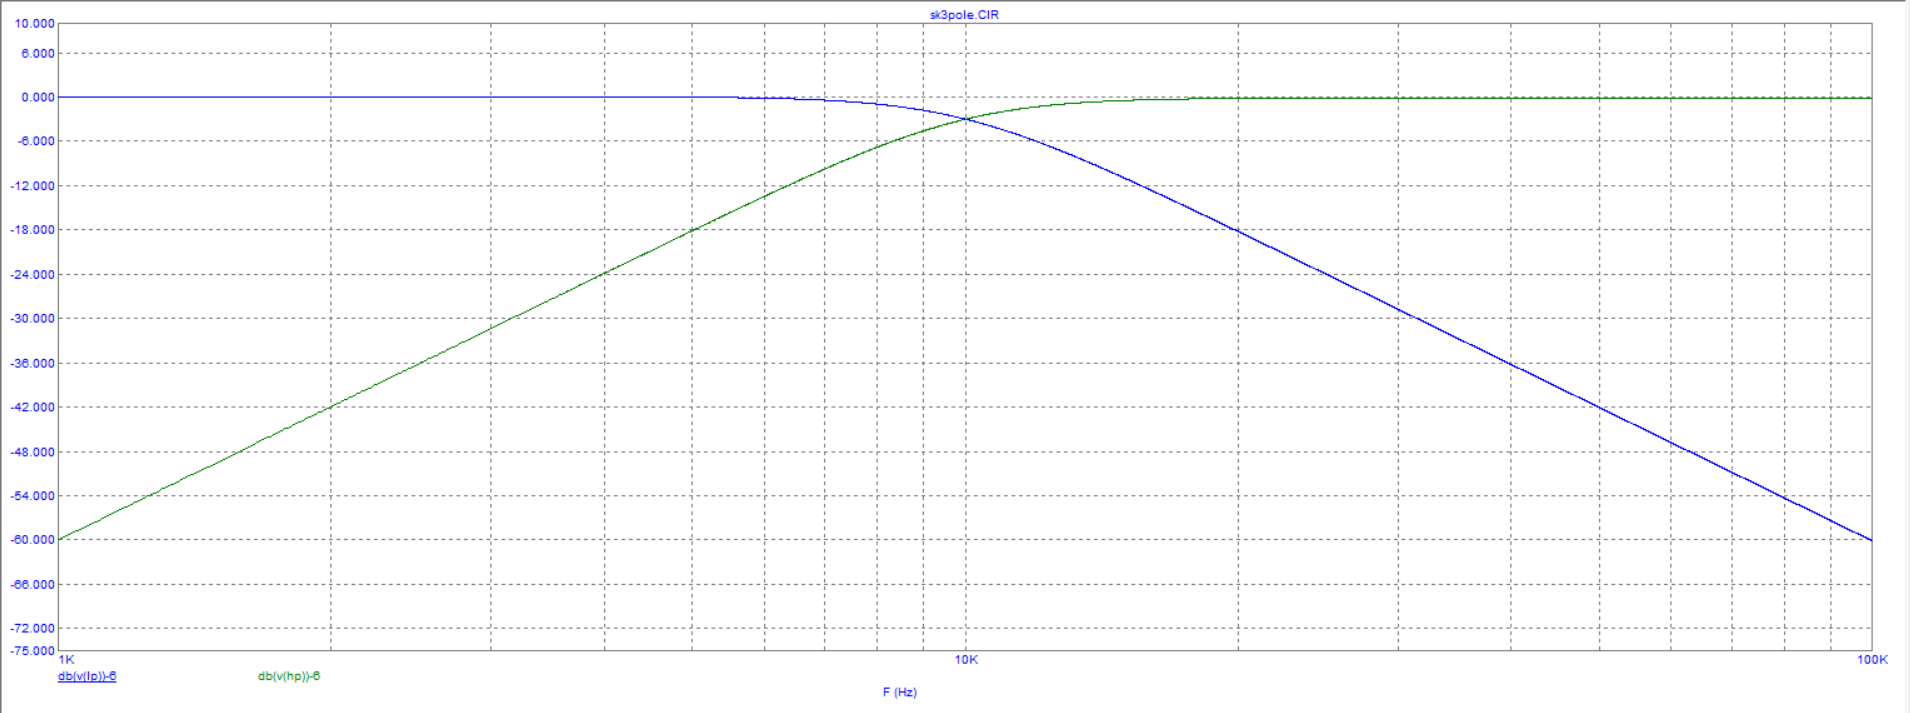
\includegraphics[width=12cm]{pics/point4_3.png}
    \caption{Варьирование $R_B  = 11K, 19K | 2K]$}
    \label{}
\end{figure}





\end{document}



 